\chapter{Methodology}
% (diagram: data flow ; from input to output, everything in between; a paragraph on each module)


\section{Machine Learning Workflow}
The Machine Learning workflow utilized during this Master thesis is based upon a universal blueprint proposed by \citet{Chollet:2017:DeepLearningPython} and will lay out how the underlying Machine Learning problem got tackled. It consists of the following 7 steps which are displayed with a few keywords describing the approach proposed by this Master thesis:

\begin{enumerate}
    \item \textbf{Defining the problem and assembling a dataset}\newline
    Emotion Recognition, Regression problem, AFEW-VA dataset
    \item \textbf{Choosing a measure of success}\newline
    RMSE, CORR
    \item \textbf{Deciding on an evaluation protocol}\newline
    5-fold-Cross-Validation
    \item \textbf{Preparing your data}\newline
    Restructure frames, Resize range of label's value
    \item \textbf{Developing a model that does better than baseline}\newline
    Implementing a first version model
    \item \textbf{Scaling up: developing a model that overfits}\newline
    Implementing the pre-trained neural network ResNet50
    \item \textbf{Regularizing your model and tuning your hyperparameters}\newline
    Dropout, DataAugmentation
\end{enumerate}



\section{Research paradigm: Ablation study}

\begin{quote}
    An Ablation Study, in medical and psychological research, is a research method in which the roles and functions of an organ, tissue, or any part of a living organism, is examined through its surgical removal and observing the behaviour of the organism in its absence.\citep{Sheikholeslami:2019:AblationProgrammingML}
\end{quote}


Ablation Study in Machine Learning is derived from its medical/psychological background and can be defined as a scientific examination of Machine Learning systems by purposefully removing features or components, in order to observe its effects on the system's performance. Thus, every design choice or module can be included in an ablation study. As a result, Ablation Study can provide valuable insights to researchers, albeit it doesn't provide sufficient proof for drawing direct conclusion on the module's contribution. \citep{Sheikholeslami:2019:AblationProgrammingML}
\newline\newline
The idea behind ablation study applied to Artificial Neural Networks (ANNs) in this Master thesis is that the network is first trained to perform its Emotion Recognition task. Afterwards, modules or design choices are removed from the network which allows the researcher to measure the performance change due to the caused damage. This paradigm will be mostly used in chapter 5.4, where experiments on top of the already developed Neural Network will be conducted. \citep{Fadelli:2018:AblationInANN}


% \subsection{Development technique: Minimum Viable Product (MVP)}
% The concept of a Minimum Viable Product (MVP) was first introduced by \citet{Ries:2011:TheLeanStartUp} as a methodology for creating a 'Lean StartUp'. It aims at starting the learning process as early as possible through integrating early adopter's feedback.\citep{Lenarduzzi:2016:MVP}
% \newline\newline
% \citet{Lenarduzzi:2016:MVP} argues that the Build-Measure-Learn loop is one of the core principles in 'Lean StartUp' which allows entrepreneurs to learn whether to give up or persevere with a current build. This build is usually defined as a MVP. The author \citet{Ries:2011:TheLeanStartUp} describes an Minimum Viable Product as follows:
% \begin{quote}
%     "The MVP is that version of the product that enables a full turn of the Build-Measure-Learn loop with a minimum amount of effort and the least amount of development time." \citep{Ries:2011:TheLeanStartUp}
% \end{quote}
% However, \citet{Ries:2011:TheLeanStartUp} clarifies that a MVP is still far from being complete, on the contrary, it requires additional effort during building as its outcomes will be presented to potential customers and its feedback needs to be measurable. 
% \newline\newline
% The MVP for this this starts off with just the code for training a artificial neural network and testing its achievements on previously unseen data. This allowed the author to show a fully functioning product from the beginning on and to add functionality with the progress of the experiments.
% \newline\newline
% While the MVP is being expanded the measurable results are being presented continually to the supervisors from the University of Hamburg, as well as the supervisor from PPI AG. The resulting feedback flows back into the product by the design of the future experiments and changes. Thus, following the philosophy of the MVP, allowed the author to steer the direction of the experiments as needed and to continually receive actionable feedback on the current state of the product.

    
%%%%%%%%%%%%%%%%%%%%%%%%%%%%%%%%%%%%%%%%%%%%%%%%%%%%%


\section{Methods}	

The approach proposed in this Master thesis is comprised of multiple methods which are illustrated in the following figure \ref{fig:MachineLearningModelMethods}. On the left hand side of the figure, a summary of the approach is illustrated in a consecutive order from top to bottom. Each important step has a number assigned to it which can be found on the right hand side with a corresponding example picture of the output of this step.

\begin{figure}[H]
  \begin{center}
  \makebox[\textwidth][c]{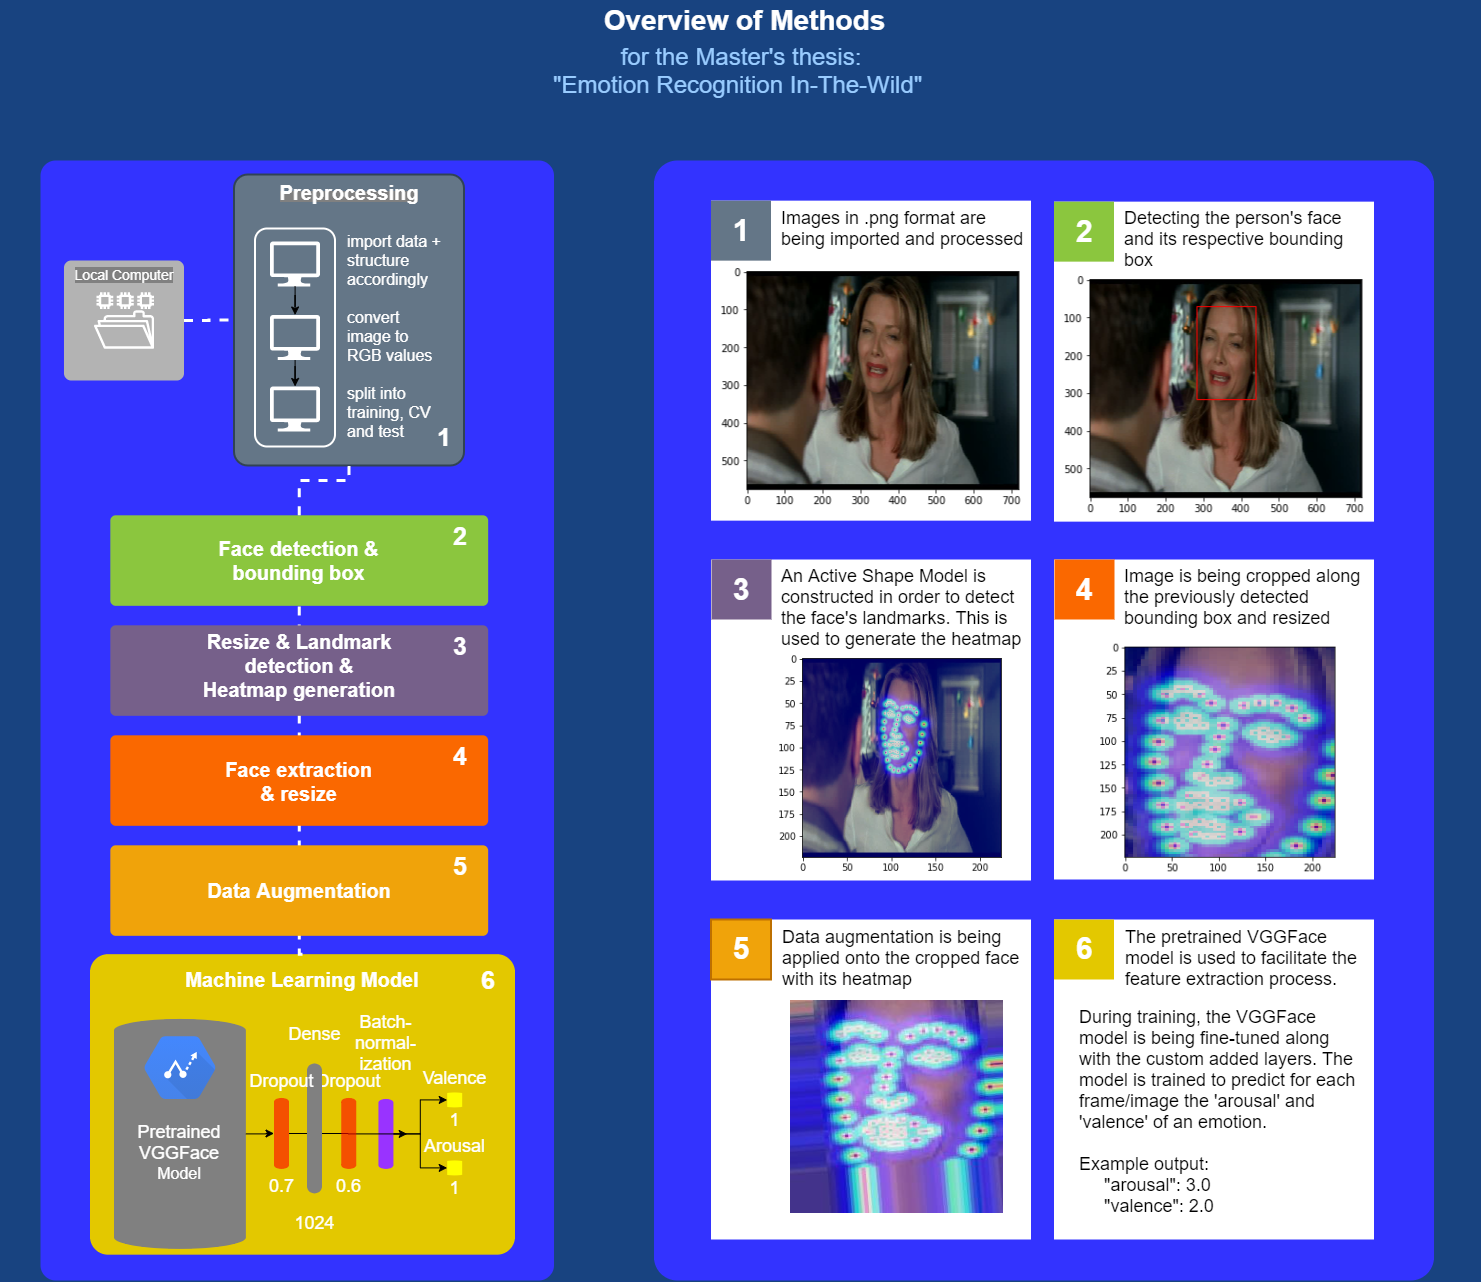
\includegraphics[width=1.2\textwidth]{Figures/DataFlow_Diagram.png}}%
  %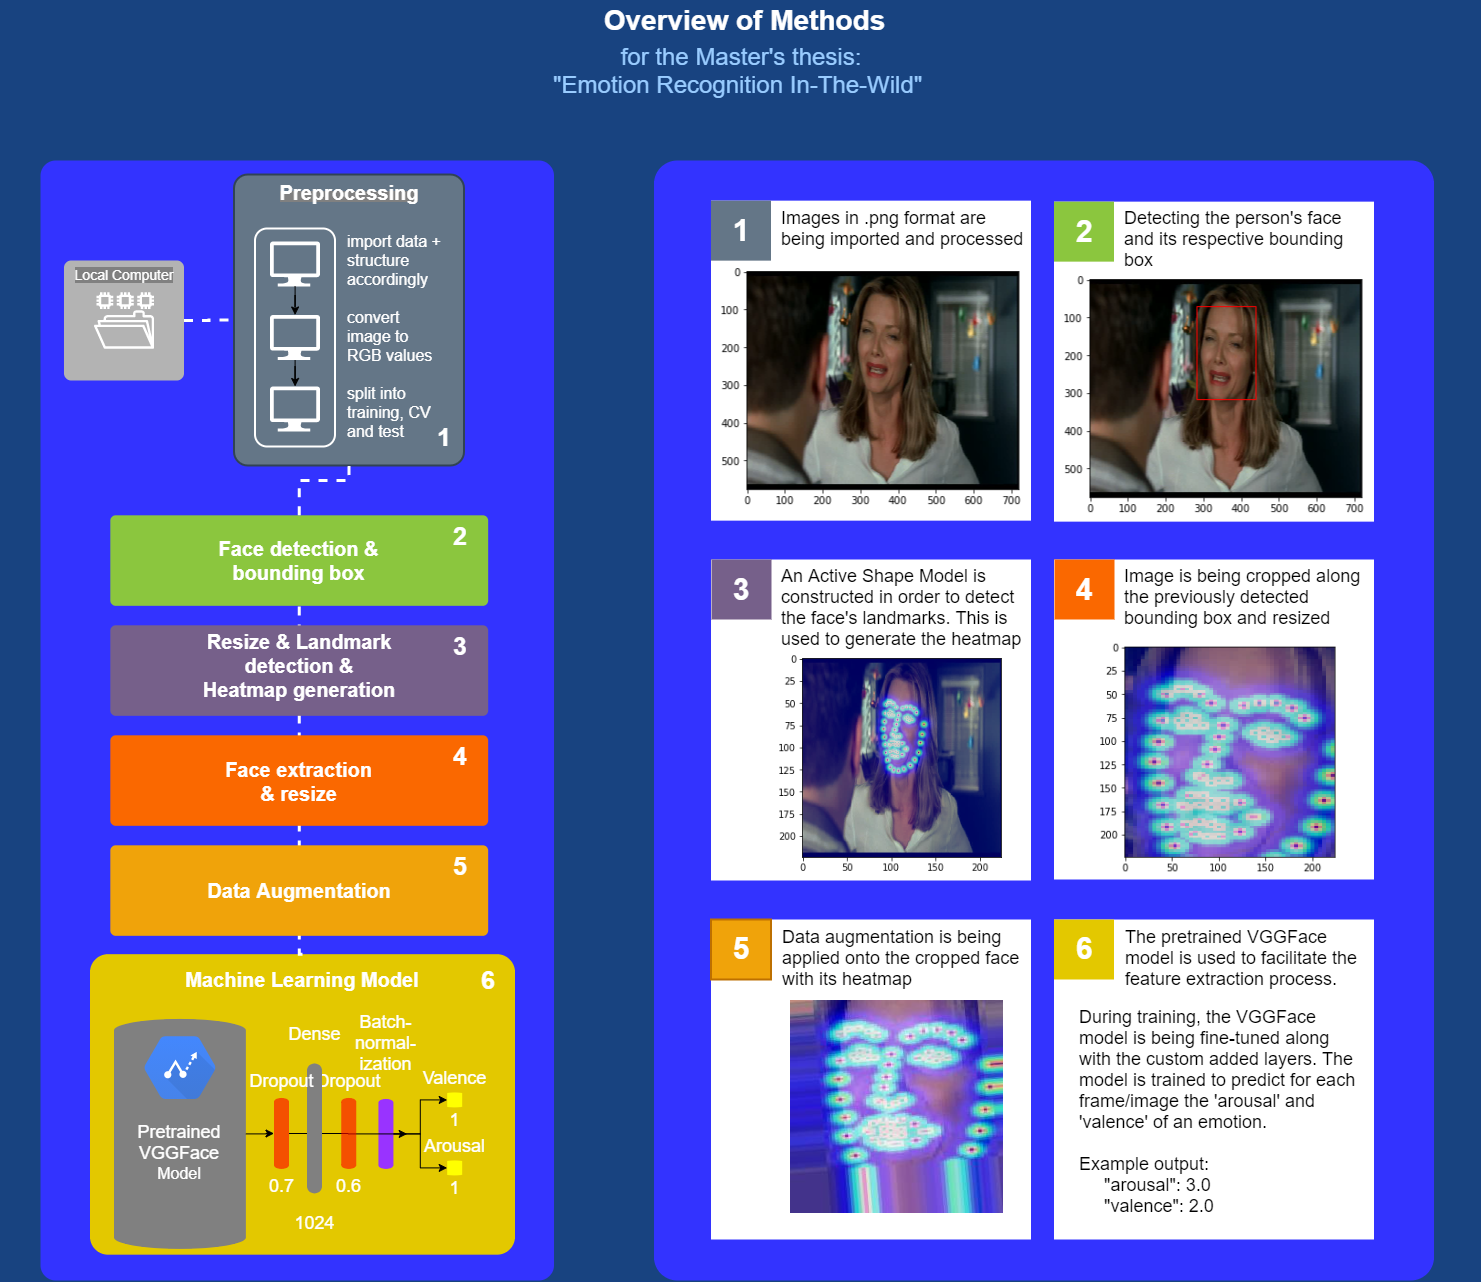
\includegraphics[angle=0, width=1.0\textwidth]{Figures/DataFlow_Diagram.png}
  \caption{Overview: Machine Learning Model - Methods}
  \label{fig:MachineLearningModelMethods}
  \end{center}
\end{figure}




\subsection{Preprocessing}
First of all, the data structure of the selected database needs to be analyzed and according to this structure data is being imported and structured. A list of all the filenames of the images and their respective labels for valence and arousal is created for each, the training and testing data. While the training data set is being shuffled for a better generalization during training, the testing data is used for validating the training results on a previously unseen part of the dataset.
\newline\newline
Based upon the list of filenames the actual image data is being read in and converted into RGB values. Furthermore, the values of valence and arousal are divided by 10, as the labels need to be brought into a range of -1 to 1 in order to fit the 'tanh' activation function of the model's final output layer.
\newline\newline
The labels and image data used for training are subsequently split into 80 \% training and 20 \% cross-validation data. 
% The last preprocessing step involves loading all the images, converting it into RGB values and then extracting the face while using the face detection techniques described in the next chapter. The cropped output image will have a shape of 224x224x3 and will be permanently saved so that this step doesn't have to be repeated each time the model is being trained. Furthermore, the model can then reach back to this array of extracted images and directly use them to train or finetune the model.

\begin{center}
\begin{figure}[H]
  \begin{center}
  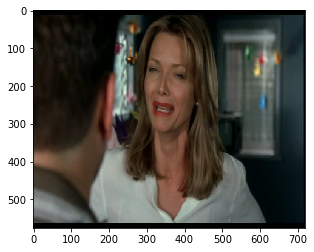
\includegraphics[angle=0, width=0.5\textwidth]{Figures/method_1.png}
  \caption{Method 1}
  \label{fig:MachineLearningModelMethod_1}
  \end{center}
\end{figure}
\end{center}


\subsection{Face detection \& bounding box}
The \gls{MTCNN} poroposed by \citet{Zhang:2016:MTCCN} is a pre-trained neural network optimized for the tasks of simultaneous face detection, face alignment, bounding boxing and landmark detection.\citep{Brownlee:2019:VggFace2HowToFaceRec}
\newline\newline
In this Master thesis, the \gls{MTCNN} model was used to detect the face in an image and determine it's coordinates for the bounding box. Thus, after a new image was read in and converted into RGB color values, the \gls{MTCNN} module can detect the face and determine its bounding box. With the bounding box coordinates a rectangle is being drawn on the input image and saved for further processing.

\begin{center}
\begin{figure}[H]
  \begin{center}
  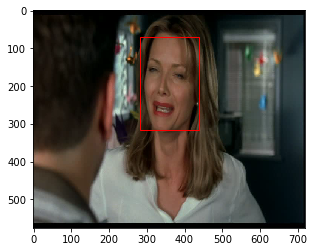
\includegraphics[angle=0, width=0.5\textwidth]{Figures/method_2.png}
  \caption{Method 2}
  \label{fig:MachineLearningModelMethod_2}
  \end{center}
\end{figure}
\end{center}

\subsection{Landmark detection \& Heatmap generation}
For the detection of landmarks the 'Face Landmark Detection' algorithm from the dlib library is implemented. This algorithm creates a shape model which it is aligning to the face at hand by refining its positions through a cascade of regressors. Additionally, dlib offers an already pre-trained version of their 'Face Landmark Detection' algorithm as a pre-trained shape predictor that can determine 68 facial landmarks.\citep{Kazemi:2014:ShapePredictor}
\newline\newline
For the implementation, the shape predictor requires, next to the input image, the bounding box of the person's face appearing in the input image. As the bounding box was already determined during the previous step by the \gls{MTCNN} module it can be directly used as an input for the landmark detection. \citep{Datahacker:2020:DlibFacialLandmarks}
\newline\newline

\begin{quote}
    imgaug is a library for image augmentation in machine learning experiments. It supports a wide range of augmentation techniques ... it can not only augment images, but also keypoints/landmarks, bounding boxes, heatmaps and segmentation maps. \citep{Jung:2020:Imgaug}
\end{quote}
For the proposed approach, imgaug was used to convert the previously detected landmarks into an heatmap and apply it as an overly onto the image.

\begin{center}
\begin{figure}[H]
  \begin{center}
  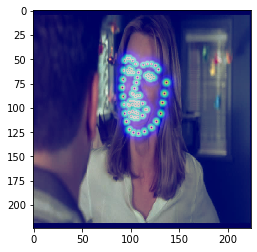
\includegraphics[angle=0, width=0.5\textwidth]{Figures/method_3.png}
  \caption{Method 3}
  \label{fig:MachineLearningModelMethod_3}
  \end{center}
\end{figure}
\end{center}

\subsection{Face extraction}
The input for this step consists of the image with a heatmap as an overlay and the coordinates for the face's bounding box. Thus, the face is simply cropped along the lines of the rectangle, comprised by the bounding boxe's coordinates. % \citep{Brownlee:2019:VggFace2HowToFaceRec}

\begin{center}
\begin{figure}[H]
  \begin{center}
  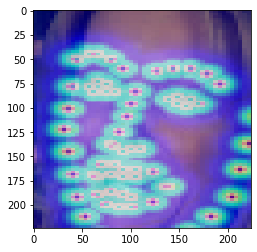
\includegraphics[angle=0, width=0.5\textwidth]{Figures/method_4.png}
  \caption{Method 4}
  \label{fig:MachineLearningModelMethod_4}
  \end{center}
\end{figure}
\end{center}

\subsection{Data Augmentation}
In order to make my model generalize better, Data Augmentation is being aplied beforehand to the pictures themselves using the ImageDataGenerator provided by Keras. It works as follows:
\begin{itemize}
    \item Taking a batch of images
    \item Apply random transformations on it
    \item Replace the original batch with the newly transformed batch
\end{itemize}
For this proposed approach data is being transformed randomly in terms of rotation, width shift, height shift, horizontal flip, brightness and zoom.

\begin{center}
\begin{figure}[H]
  \begin{center}
  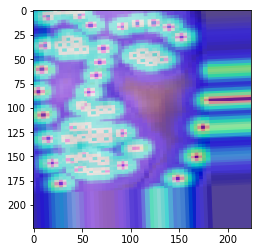
\includegraphics[angle=0, width=0.5\textwidth]{Figures/method_5.png}
  \caption{Method 5}
  \label{fig:MachineLearningModelMethod_5}
  \end{center}
\end{figure}
\end{center}


\subsection{Machine Learning Model for Emotion Recognition}
In order to get a state-of-the-art Machine Learning model for Emotion Recognition, the author decided to make use of a pre-trained model that was already trained to solve a similar challenge and fine-tune it then. 
\newline\newline
The decision fell on the VGGFace Model which is optimized for face recognition and was pre-trained on a large-scale face dataset named VGGFace2. The dataset contains about 3.31 million images of 9131 subjects and poses additionally a great variety in pose, age, etc. The architecture used for the VGGFace Model is a ResNet-50 Convolutional Neural Network that was trained on the VGGFace2 dataset for the purpose of face recognition. When the VGGFace2 paper\citet{Cao:2018:VGGFace2} was published in \citeyear{Cao:2018:VGGFace2}, its performance exceeded the pevious state-of-the-art by a large margin. \citep{Cao:2018:VGGFace2}
\newline\newline
Due to the fact, that VGGFace is optimized for face recognition it had to learn similar facial features to what is needed by emotion recognition. Therefore, the VGGFace model's main selling point is that it already learned how to extract facial features from an image. However, the last Dense layers of the model cannot be reused as they are trimmed to learn the connection between facial features and the output of the face recognition challenge. As a result, the last Dense layers are replaced by custom made layers which consist of a Dropout layer, a single Dense layer with 1024 units, another Dropout layer, a Batch Normalization layer and two Dense layers, one for each output value.
\newline\newline
Using the above described architecture, finetuning needs to be conducted in order to fit the pre-trained model better to the Emotion Recognition challenge at hand. This means, that the weights of the pre-trained model are used as a basis for training on the AFEW-VA dataset with its images and respective labels.